\section{Materiais e Métodos}

\subsection{Descrição do problema}
No capítulo \ref{chap1} foi apresentado um problema magnético. Nele, um núcleo de chapas de aço era percorrido por um enrolamento que por sua vez era excitado com uma tensão à 60hz. Foram observados a densidade de fluxo magnético, o potencial elétrico e a intensidade de campo ao longo do núcleo magnético. O desenho do objeto, a definição dos materiais, a característica elétrica do circuito e outros parâmetros foram definidas no FEMM. Este capítulo apresenta o emprego da linguagem LUA para executar as tarefas realizadas na interface do aplicativo FEMM, conforme descrito no capítulo anterior.

\subsection{Ferramenta de elementos finitos: FEMM}
FEMM (Finite Elements Method Magnetics) é um conjunto de programas utilizados para a resolução de problemas eletromagnéticos de baixa frequência em domínios planares (bidimensional) ou assimétricos. O problema permite a resolução dos seguintes tipos de problemas: magnéticos lineares/não-lineares, problemas eletroestáticos lineares, problemas de fluxo de calor e problemas de fluxo de corrente \cite{Meeker2014}.

\subsection{Comandos para FEMM-Lua}
Comandos básicos para o FEMM-LUA:
\begin{itemize}
  \item \textbf{clearconsole()}: Limpa a janela de saída;
  \item \textbf{newdocument()}: Cria um novo documento pré-processador;
  \item \textbf{print()}: Comando de saída para envio de mensagem;
  \item \textbf{quit()}: Fecha todos os documentos e sai da camada de interação;
  \item \textbf{mi\_probdeb()}: Definições do problema (Frequência, unidade, tipo do problema, precisão, entre outros.);
\end{itemize}
%
%Comandos para adicionar/remover/editar objetos, materiais, blocos, entre outros:
\begin{itemize}
  \item \textbf{mi\_addnode(x,y)}: Adiciona um nó na coordenada x,y.
  \item \textbf{mi\_addsegment(x1,y1,x2,y2)}: Adiciona um segmento de linha entre os nós localizados em (x1,y1) e (x2,y2).
  \item \textbf{mi\_addarc(x1,y1,x2,y2,Â)}: Adiciona um arco de ângulo  entre os nós localizados em (x1,y1) e (x2,y2).
  \item \textbf{mi\_selectsegment(x,y)}: Seleciona o segmento compreendido entre os pontos x e y).
  \item \textbf{mi\_getmaterial()}: Adiciona um item para a lista de materiais.
  \item \textbf{mi\_addcircprop(A,B,C)}: Adiciona um circuito (A: nome do circuito, B: valor da corrente: C: 0 (paralelo) ou 1 (série)).
  \item \textbf{mi\_addblocklabel(x,y)}: Adiciona um bloco localizado na posição (x,y).
\end{itemize}
%
%Comandos para criar malha de pontos (triângulação), gerar gráficos, entre outros:
\begin{itemize}
  \item \textbf{mi\_createmesh()}: Executa triangulação.
  \item \textbf{mi\_loadsolution()}: Carrega e executa a solução correspondente ao objeto em seleção.
	\item \textbf{mo\_showdensityplot()}: Gera gráfico de densidade de fluxo.
  \item \textbf{mo\_makeplot()}: Gera um gráfico definido (Exemplos: 0-Potencial; 1-|B|; 3-|H|).
\end{itemize}

\subsection{Ferramenta para processar arquivo .LUA no FEMM}
\begin{figure}[h]
\centering
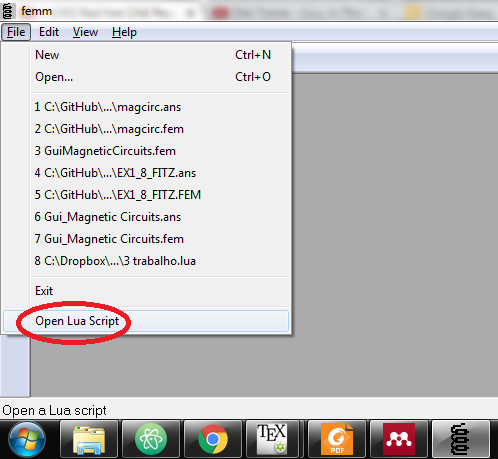
\includegraphics[scale=1]{img/assig2/open_lua_script.png}
\caption[Carregar arquivo script LUA]{Carregar arquivo script LUA.}
\label{circ}
\end{figure}
